\documentclass[crop,tikz,border=1px]{standalone}

\usetikzlibrary{arrows,positioning,scopes,automata,calc}

\begin{document}
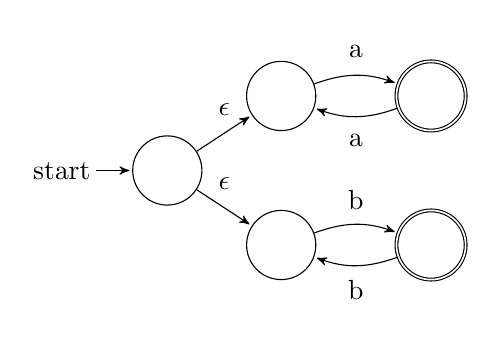
\begin{tikzpicture}[->,>=stealth',shorten >=1pt,auto,
  inner sep=2pt,minimum size=.6cm,
  mystate/.style={state,text centered}]

  \node[mystate] (qa1)  {};
  \node[mystate] (qb1) [below=of qa1] {};
  \coordinate (mid) at ($(qa1)!0.5!(qb1)$);
  \node[initial,mystate] (q0) [left=of mid] {};
  \node[accepting,mystate] (qa2) [right=of qa1] {};
  \node[accepting,mystate] (qb2) [right=of qb1] {};

  \path (q0) edge node [above] {\(\epsilon\)} (qa1)
        (q0) edge node [above] {\(\epsilon\)} (qb1);

  {[every edge/.append style={bend left=20}]
    \path (qa1) edge node [above] {a} (qa2)
          (qa2) edge node [below] {a} (qa1)

          (qb1) edge node [above] {b} (qb2)
          (qb2) edge node [below] {b} (qb1);
  }

\end{tikzpicture}
\end{document}
